\documentclass[12pt,a4paper]{article}

% ---------- Packages ----------
\usepackage[margin=1in]{geometry}
\usepackage{graphicx}
\usepackage{booktabs}
\usepackage{longtable}
\usepackage{array}
\usepackage{amsmath}
\usepackage{hyperref}
\usepackage{enumitem}
\usepackage{fancyhdr}
\usepackage{xcolor}
\usepackage{titlesec}
\usepackage{float}
\usepackage{setspace}
% Shared LaTeX preamble for all Data Mining / ISLR chapter documents.
% Provides \makecoverpage{<assignment title>} — a standalone title page
% with fixed student identity, so every chapter/lab looks uniform.

\usepackage{graphicx}

\newcommand{\makecoverpage}[1]{%
\begin{titlepage}
\centering
\vspace*{2cm}

{\Large \textbf{Adventist University of Central Africa}}\\[0.4cm]
{\large Master's in Big Data Analytics}\\[2cm]

{\Huge \textbf{#1}}\\[0.5cm]
{\large \textit{Introduction to Statistical Learning with Applications in R}}\\[3cm]

\begin{tabular}{rl}
\textbf{Programme:} & MSc Big Data Analytics \\
\textbf{Course Title:} & Data Mining \\
\textbf{Course Code:} & MSDA 9124 \\
\textbf{Lecturer:} & Dr. Pacifique Nizeyimana \\
\textbf{Student Name:} & Wayne Rubangisa \\
\textbf{Student ID:} & 101220 \\
\end{tabular}

\vfill

{\large September 2026}

\end{titlepage}
}

\newcommand{\TransactionCount}{9835}
\newcommand{\UniqueItemCount}{169}
\newcommand{\ItemsetCount}{63}
\newcommand{\RuleCount}{49}
\newcommand{\MinSupport}{0.02}
\newcommand{\MinConfidence}{0.25}
\newcommand{\TopConfidenceRule}{\{other vegetables,yogurt\} $\Rightarrow$ \{whole milk\}}
\newcommand{\TopConfidenceValue}{0.5129}
\newcommand{\TopLiftRule}{\{other vegetables,whole milk\} $\Rightarrow$ \{root vegetables\}}
\newcommand{\TopLiftValue}{2.8421}
\newcommand{\TopSupportRule}{\{other vegetables\} $\Rightarrow$ \{whole milk\}}
\newcommand{\TopSupportValue}{0.0748}


\onehalfspacing

\hypersetup{
  colorlinks=true,
  linkcolor=blue!50!black,
  urlcolor=blue!50!black,
  citecolor=blue!50!black
}

\titleformat{\section}{\large\bfseries}{Q\arabic{section}.}{0.5em}{}
\titleformat{\subsection}{\normalsize\bfseries}{(\alph{subsection})}{0.5em}{}

\pagestyle{fancy}
\fancyhf{}
\rhead{Association Rule Learning -- Groceries Dataset}
\lhead{\thepage}
\renewcommand{\headrulewidth}{0.3pt}

\setlength{\parskip}{0.5em}
\setlength{\parindent}{0pt}

\begin{document}

\makecoverpage{Association Rule Learning \\ Groceries Dataset}

\pagenumbering{roman}
\tableofcontents
\newpage
\pagenumbering{arabic}

\subsection{Why these thresholds were chosen}
The minimum support of \textbf{\MinSupport} keeps the analysis focused on itemsets that
appear in a meaningful share of the \TransactionCount transactions. The minimum confidence
of \textbf{\MinConfidence} removes rules that make weak predictions about their consequent.
These are practical screening thresholds, not universal statistical cutoffs. Lowering either
threshold would produce more rules, including rarer and potentially less stable patterns;
raising them would produce a shorter list focused on the most common relationships. The
thresholds should therefore be interpreted together with support, confidence, and lift rather
than as evidence that every retained rule is important.

% ================= BODY =================

	extbf{\TopConfidenceRule}, confidence = \textbf{\TopConfidenceValue}

\subsection{Number of transactions}
	extbf{\TopLiftRule}, lift = \textbf{\TopLiftValue}
market basket.

	extbf{\TopSupportRule}, support = \textbf{\TopSupportValue}
The dataset contains \textbf{\UniqueItemCount unique grocery items}.

\subsection{Ten most frequently purchased items}

Table~\ref{tab:top10} and Figure~\ref{fig:top10} show the ten items with the highest support
(relative purchase frequency).

\begin{table}[H]
\centering
\caption{Top 10 most frequent items}
\label{tab:top10}
\begin{tabular}{lrr}
\toprule
\textbf{Item} & \textbf{Support} & \textbf{Count} \\
\midrule
Whole milk         & 0.2555 & 2{,}513 \\
Other vegetables   & 0.1935 & 1{,}903 \\
Rolls/buns         & 0.1839 & 1{,}809 \\
Soda               & 0.1744 & 1{,}715 \\
Yogurt             & 0.1395 & 1{,}372 \\
Bottled water      & 0.1105 & 1{,}087 \\
Root vegetables    & 0.1090 & 1{,}072 \\
Tropical fruit     & 0.1049 & 1{,}032 \\
Shopping bags      & 0.0985 &   969 \\
Sausage            & 0.0940 &   924 \\
\bottomrule
\end{tabular}
\end{table}

\begin{figure}[H]
\centering
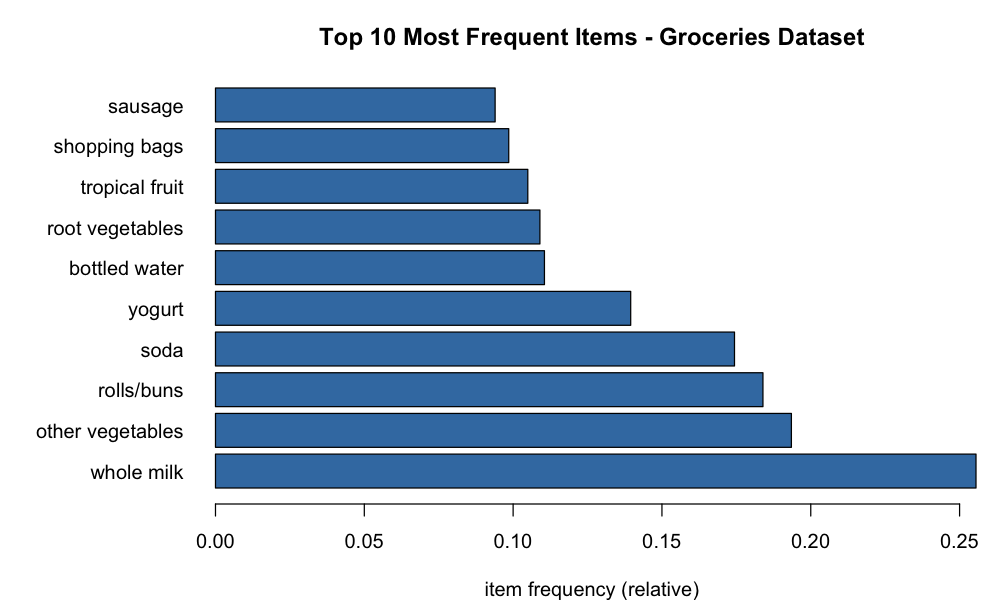
\includegraphics[width=0.85\textwidth]{../results/top10_items.png}
\caption{Top 10 most frequent items by support}
\label{fig:top10}
\end{figure}

Whole milk and other vegetables are, by a clear margin, the two staples of this store's
customer base -- unsurprising, since both are everyday perishables bought on nearly every
shopping trip.

\clearpage
\section{Frequent Itemsets}

\subsection{At least 10 frequent itemsets (two or more products)}

Using a minimum support threshold of \textbf{0.02} (i.e.\ the itemset appears in at least
2\% of all transactions) and a minimum itemset size of 2, the analysis identified
\textbf{\ItemsetCount frequent itemsets} (61 pairs and 2 triples). Table~\ref{tab:itemsets} lists the
top 10 by support.

\begin{table}[H]
\centering
\caption{Top 10 frequent itemsets by support}
\label{tab:itemsets}
\begin{tabular}{lrr}
\toprule
\textbf{Itemset} & \textbf{Support} & \textbf{Count} \\
\midrule
\{other vegetables, whole milk\}        & 0.0748 & 736 \\
\{rolls/buns, whole milk\}              & 0.0566 & 557 \\
\{whole milk, yogurt\}                  & 0.0560 & 551 \\
\{root vegetables, whole milk\}         & 0.0489 & 481 \\
\{other vegetables, root vegetables\}   & 0.0474 & 466 \\
\{other vegetables, yogurt\}            & 0.0434 & 427 \\
\{other vegetables, rolls/buns\}        & 0.0426 & 419 \\
\{tropical fruit, whole milk\}          & 0.0423 & 416 \\
\{soda, whole milk\}                    & 0.0401 & 394 \\
\{rolls/buns, soda\}                    & 0.0383 & 377 \\
\bottomrule
\end{tabular}
\end{table}

\subsection{Support values}
Support values are reported directly in Table~\ref{tab:itemsets} (column \emph{Support}),
ranging from 0.0383 to 0.0748 for the top 10 itemsets.

\subsection{Highest-support itemset}
\{other vegetables, whole milk\} has the highest support at \textbf{0.0748} (736 of 9{,}835
transactions) -- almost twice the support of the next-highest itemset.

\subsection{What support tells us about purchasing behavior}
Support measures how common an itemset is across \emph{all} transactions, regardless of
what else is happening in the basket. A support of 0.0748 for \{other vegetables, whole
milk\} means that roughly 1 in 13 shopping trips includes both items together. High-support
itemsets identify the combinations that matter at scale -- store layout, staffing, and
inventory decisions built around them affect a large share of all customers, whereas a
rule with strong confidence but tiny support only describes a small, possibly niche, slice
of shoppers.

\clearpage
\section{Association Rules}

\subsubsection*{Measures used}
Three measures are used throughout this report, for a rule $A \Rightarrow B$ and an
itemset $X$ (with $T$ the set of all transactions):

\[
\text{support}(X) = \frac{|\{t \in T : X \subseteq t\}|}{|T|}
\qquad
\text{confidence}(A \Rightarrow B) = \frac{\text{support}(A \cup B)}{\text{support}(A)}
\qquad
\text{lift}(A \Rightarrow B) = \frac{\text{confidence}(A \Rightarrow B)}{\text{support}(B)}
\]

\subsection{At least 10 association rules}

Rules were generated from the frequent itemsets above using a minimum confidence of
\textbf{\MinConfidence}, yielding \textbf{\RuleCount rules} in total. Table~\ref{tab:rules} lists the top 12,
sorted by lift.

\begin{table}[H]
\centering
\caption{Association rules (sorted by lift)}
\label{tab:rules}
\resizebox{\textwidth}{!}{%
\begin{tabular}{llrrr}
\toprule
\textbf{Antecedent} & \textbf{Consequent} & \textbf{Support} & \textbf{Confidence} & \textbf{Lift} \\
\midrule
other vegetables, whole milk & root vegetables    & 0.0232 & 0.3098 & 2.8421 \\
pip fruit                    & tropical fruit     & 0.0204 & 0.2702 & 2.5746 \\
root vegetables, whole milk  & other vegetables   & 0.0232 & 0.4740 & 2.4498 \\
root vegetables              & other vegetables   & 0.0474 & 0.4347 & 2.2466 \\
other vegetables, whole milk & yogurt             & 0.0223 & 0.2976 & 2.1330 \\
whipped/sour cream           & other vegetables   & 0.0289 & 0.4028 & 2.0819 \\
whipped/sour cream           & yogurt             & 0.0207 & 0.2894 & 2.0743 \\
whole milk, yogurt           & other vegetables   & 0.0223 & 0.3975 & 2.0541 \\
other vegetables, yogurt     & whole milk         & 0.0223 & 0.5129 & 2.0072 \\
tropical fruit                & yogurt            & 0.0293 & 0.2791 & 2.0005 \\
butter                       & whole milk         & 0.0276 & 0.4972 & 1.9461 \\
pork                         & other vegetables   & 0.0217 & 0.3757 & 1.9415 \\
\bottomrule
\end{tabular}}
\end{table}

\begin{figure}[H]
\centering
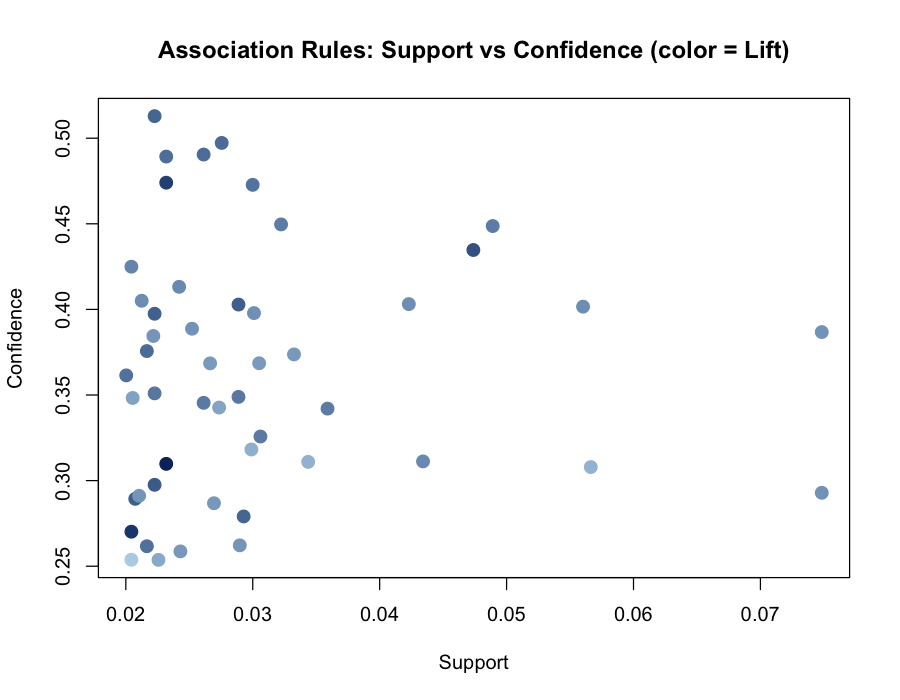
\includegraphics[width=0.75\textwidth]{../results/rules_scatter.png}
\caption{All 49 rules: support vs.\ confidence, coloured by lift (darker = higher lift)}
\label{fig:scatter}
\end{figure}

\clearpage
\section{Understanding the Measures}

Three rules from Table~\ref{tab:rules} are examined below.

\subsection{Support}
\begin{itemize}[leftmargin=1.2em]
  \item \textbf{\{other vegetables, whole milk\} $\rightarrow$ \{root vegetables\}}:
  \[
  \text{support} = \frac{|\{t : \{\text{o.veg, milk, root veg}\} \subseteq t\}|}{9{,}835}
  = \frac{228}{9{,}835} = 0.0232
  \]
  this exact combination of all three items occurs in 2.32\% of all
  transactions.
  \item \textbf{\{root vegetables\} $\rightarrow$ \{other vegetables\}}: support = 0.0474 --
  both items together appear in 4.74\% of transactions.
  \item \textbf{\{butter\} $\rightarrow$ \{whole milk\}}: support = 0.0276 -- both items
  appear together in 2.76\% of transactions.
\end{itemize}

\subsection{Confidence}
\begin{itemize}[leftmargin=1.2em]
  \item \textbf{\{other vegetables, whole milk\} $\rightarrow$ \{root vegetables\}}:
  \[
  \text{confidence} = \frac{\text{support}(A \cup B)}{\text{support}(A)}
  = \frac{0.0232}{0.0748} = 0.3098
  \]
  of the customers who bought other vegetables \emph{and} whole
  milk, 30.98\% also bought root vegetables.
  \item \textbf{\{root vegetables\} $\rightarrow$ \{other vegetables\}}: confidence =
  0.4347 -- 43.47\% of customers who bought root vegetables also bought other vegetables.
  \item \textbf{\{butter\} $\rightarrow$ \{whole milk\}}: confidence = 0.4972 -- almost half
  (49.72\%) of butter buyers also bought whole milk.
\end{itemize}

\subsection{Lift}
\begin{itemize}[leftmargin=1.2em]
  \item \textbf{\{other vegetables, whole milk\} $\rightarrow$ \{root vegetables\}}:
  \[
  \text{lift} = \frac{\text{confidence}(A \Rightarrow B)}{\text{support}(B)}
  = \frac{0.3098}{0.1090} = 2.8421
  \]
  customers who buy other vegetables and whole milk are 2.84 times more likely to
  also buy root vegetables than a random customer.
  \item \textbf{\{root vegetables\} $\rightarrow$ \{other vegetables\}}: lift = 2.25 --
  buying root vegetables makes buying other vegetables 2.25 times more likely than chance.
  \item \textbf{\{butter\} $\rightarrow$ \{whole milk\}}: lift = 1.95 -- buying butter
  makes buying whole milk about 1.95 times more likely than chance, despite whole milk
  already being the most popular item in the store.
\end{itemize}

\clearpage
\section{Find Interesting Rules}

\subsection{Highest confidence}
\textbf{\{other vegetables, yogurt\} $\rightarrow$ \{whole milk\}}, confidence = 0.5129
(support = 0.0223, lift = 2.01).

\subsection{Highest lift}
\textbf{\{other vegetables, whole milk\} $\rightarrow$ \{root vegetables\}}, lift = 2.84
(support = 0.0232, confidence = 0.31).

\subsection{Highest support}
\textbf{\{other vegetables\} $\rightarrow$ \{whole milk\}}, support = 0.0748
(confidence = 0.3868, lift = 1.51).

\subsection{Are these the same rule?}
No -- all three are different rules. This is expected: support rewards
\emph{popularity} (the highest-support rule involves the two most common items in the
store, so it occurs often even though the association is only moderately strong -- lift
1.51 is the lowest of the three). Confidence rewards \emph{reliability} of the antecedent
predicting the consequent, which is why the highest-confidence rule points at whole milk,
the single most-bought item overall -- it's an easy consequent to satisfy. Lift rewards
\emph{genuine association strength} after removing the effect of overall popularity, which
is why the highest-lift rule involves root vegetables, a less common item whose purchase is
still strongly tied to a specific combination of other items. A rule can score well on one
measure and only moderately on the others, since each measure is answering a different
question.

\clearpage
\section{Interpret a Rule}

Selected rule: \textbf{\{other vegetables, whole milk\} $\rightarrow$ \{root vegetables\}}
(support = 0.0232, confidence = 0.31, lift = 2.84).

\textbf{In simple language:} Customers who purchase other vegetables and whole milk in the
same trip also tend to purchase root vegetables in about 31\% of those trips -- noticeably
more often than root vegetables are bought overall (support 0.109), which is exactly what
the lift of 2.84 captures.

\textbf{Strong or weak association?} This rule represents a \textbf{moderately strong}
association. The lift of 2.84 is comfortably above 1, meaning the three items co-occur far
more than chance would predict, and 31\% confidence means nearly a third of the relevant
customers follow the pattern. It is not an overwhelming rule (confidence is well under 50\%),
but combined with a lift close to 3, it is one of the more meaningful relationships found in
this dataset -- plausibly reflecting a shared "cooking a vegetable-based meal" shopping
occasion.

\clearpage
\section{Business Application}

Imagine acting as the supermarket manager, using the rules above.

\subsection{Two products to place close together}
\textbf{Root vegetables and other vegetables.} Their rule (\{root vegetables\}
$\rightarrow$ \{other vegetables\}, lift = 2.25) shows a strong, high-confidence
association (43.5\%), and both are fresh produce that is naturally merchandised in the
same aisle already -- placing them adjacent (or cross-merchandising root vegetables at the
front of the vegetable section) would shorten the trip for a large share of customers.

\subsection{One possible product bundle}
A \textbf{"vegetable basket" bundle of other vegetables + whole milk + root vegetables}
(the highest-lift itemset, lift 2.84) -- e.g.\ a discounted "dinner veg box" combining
these three -- targets an already-existing shopping pattern rather than trying to create
a new one.

\subsection{Using association rules for recommendations}
At checkout (in-store) or in an online cart, the system could flag: "Customers who bought
other vegetables and whole milk also bought root vegetables (frequently)" and offer a small
discount or a reminder nudge -- a "you might also need" prompt driven directly by the rule
\{other vegetables, whole milk\} $\rightarrow$ \{root vegetables\}, rather than a generic or
manually curated suggestion.

\clearpage
\section{Understanding Association}

\subsection{Does an association rule prove causation?}
No. An association rule only describes \textbf{co-occurrence} in the transaction data --
that customers who bought $A$ frequently also bought $B$. It says nothing about
\emph{why}: $A$ might not cause anyone to buy $B$ at all. Both could be driven by a
common cause (e.g.\ both are ingredients for the same popular recipe), by seasonality, by
store layout placing them near each other, or by pure coincidence in a large dataset.
Confirming causation would require a controlled experiment (e.g.\ moving product placement
and measuring the effect), not just mining historical baskets.

\subsection{High confidence but low lift}
This happens when the consequent is already very common on its own. Confidence only asks
"given the antecedent, how often does the consequent follow?" -- if the consequent (say,
whole milk, support 0.2555) is bought in a quarter of \emph{all} transactions regardless of
anything else, then almost any antecedent will show reasonably high confidence for
predicting it, purely because it's hard to miss. Lift corrects for this by dividing by the
consequent's baseline popularity, so a rule can have confidence well above the dataset
average while still having lift close to 1 -- meaning the antecedent barely changes the
odds of the consequent compared to knowing nothing at all.

\subsection{What a lift greater than 1 indicates}
Lift $> 1$ indicates a \textbf{positive association}: the two itemsets occur together more
often than would be expected if they were purchased independently. The further above 1, the
stronger the association (lift $= 1$ means no association / statistical independence, and
lift $< 1$ indicates a negative association, where buying one item makes the other
\emph{less} likely).

\clearpage
\section{Limitations and Responsible Use}

The results describe this transaction sample under the selected thresholds; they do not
establish that the rules will hold in every store, season, or customer segment. Rare rules
are especially sensitive to a small number of baskets, and repeated searches over many
possible rules increase the chance of finding apparently impressive patterns by chance.
The analysis also treats each transaction as a basket and does not include price, quantity,
customer identity, time, promotion, or store-location information. These omitted variables
could explain part of the observed associations.

For a production recommendation system, candidate rules should therefore be tested on a
later holdout period or a different store before deployment. A/B testing product placement
or recommendation messages would be needed to estimate whether a proposed intervention
actually changes purchasing behaviour.

\subsection{Choosing a rule for a business decision}

The appropriate metric depends on the decision. High-support rules are useful for broad
inventory and store-layout decisions because they affect many baskets. High-confidence rules
are useful when the business wants a reliable follow-up recommendation after an antecedent
has already been observed. High-lift rules are useful for targeted cross-selling because they
identify combinations that are unusually strong relative to the consequent's baseline
popularity. In all three cases, the metric should be considered alongside support: a very
high lift based on only a handful of transactions may not be stable enough to act on.

\end{document}
